% Options for packages loaded elsewhere
\PassOptionsToPackage{unicode}{hyperref}
\PassOptionsToPackage{hyphens}{url}
%
\documentclass[
  12pt,
]{article}
\usepackage{amsmath,amssymb}
\usepackage{iftex}
\ifPDFTeX
  \usepackage[T1]{fontenc}
  \usepackage[utf8]{inputenc}
  \usepackage{textcomp} % provide euro and other symbols
\else % if luatex or xetex
  \usepackage{unicode-math} % this also loads fontspec
  \defaultfontfeatures{Scale=MatchLowercase}
  \defaultfontfeatures[\rmfamily]{Ligatures=TeX,Scale=1}
\fi
\usepackage{lmodern}
\ifPDFTeX\else
  % xetex/luatex font selection
\fi
% Use upquote if available, for straight quotes in verbatim environments
\IfFileExists{upquote.sty}{\usepackage{upquote}}{}
\IfFileExists{microtype.sty}{% use microtype if available
  \usepackage[]{microtype}
  \UseMicrotypeSet[protrusion]{basicmath} % disable protrusion for tt fonts
}{}
\makeatletter
\@ifundefined{KOMAClassName}{% if non-KOMA class
  \IfFileExists{parskip.sty}{%
    \usepackage{parskip}
  }{% else
    \setlength{\parindent}{0pt}
    \setlength{\parskip}{6pt plus 2pt minus 1pt}}
}{% if KOMA class
  \KOMAoptions{parskip=half}}
\makeatother
\usepackage{xcolor}
\usepackage[margin=1in]{geometry}
\usepackage{graphicx}
\makeatletter
\def\maxwidth{\ifdim\Gin@nat@width>\linewidth\linewidth\else\Gin@nat@width\fi}
\def\maxheight{\ifdim\Gin@nat@height>\textheight\textheight\else\Gin@nat@height\fi}
\makeatother
% Scale images if necessary, so that they will not overflow the page
% margins by default, and it is still possible to overwrite the defaults
% using explicit options in \includegraphics[width, height, ...]{}
\setkeys{Gin}{width=\maxwidth,height=\maxheight,keepaspectratio}
% Set default figure placement to htbp
\makeatletter
\def\fps@figure{htbp}
\makeatother
\setlength{\emergencystretch}{3em} % prevent overfull lines
\providecommand{\tightlist}{%
  \setlength{\itemsep}{0pt}\setlength{\parskip}{0pt}}
\setcounter{secnumdepth}{5}
\usepackage{setspace,lscape} \usepackage{amsmath} \usepackage{caption,subcaption,multirow} \usepackage[hang]{footmisc} \usepackage{enumitem} \usepackage{standalone} \renewcommand{\arraystretch}{1.5} \captionsetup[table]{skip=5pt} \setstretch{1.5} \setlength{\parindent}{1em} \setlength{\footnotemargin}{3mm} \setlength{\footnotesep}{3mm}
\ifLuaTeX
  \usepackage{selnolig}  % disable illegal ligatures
\fi
\usepackage[]{natbib}
\bibliographystyle{apalike}
\IfFileExists{bookmark.sty}{\usepackage{bookmark}}{\usepackage{hyperref}}
\IfFileExists{xurl.sty}{\usepackage{xurl}}{} % add URL line breaks if available
\urlstyle{same}
\hypersetup{
  pdftitle={An Attentional Model of Time Discounting},
  pdfauthor={Zark Zijian Wang},
  hidelinks,
  pdfcreator={LaTeX via pandoc}}

\title{An Attentional Model of Time Discounting}
\author{Zark Zijian Wang}
\date{June 03, 2024}

\begin{document}
\maketitle

\hypertarget{introduction}{%
\section{Introduction}\label{introduction}}

decision maker (DM)

Kullback--Leibler~(KL)~divergence~(also called~relative entropy)

hard attention

information avoidance

endogenous time preferences

optimal expectation

we present an axiomatic characterization of AAD with the optimal
discounting framework

\hypertarget{model-setting}{%
\section{Model Setting}\label{model-setting}}

Assume time is discrete. Let
\(s_{0\rightarrow T}\equiv[s_0,s_1,...,s_T]\) denote a reward sequence
that starts delivering rewards at period 0 and ends at period \(T\). At
each period \(t\) of \(s_{0\rightarrow T}\), a specific reward \(s_t\)
is delivered, where \(t\in\{0,1,…,T\}\). Throughout this paper, we only
consider non-negative rewards and finite length of sequence, i.e.~we set
\(s_t \in \mathbb{R}_{\geq 0}\) and \(1\leq T<\infty\). The DM's choice
set is constituted by a range of alternative reward sequences which
start from period 0 and end at some finite period. When making an
intertemporal choice, the DM seeks to find a reward sequence
\(s_{0\rightarrow T}\) in her choice set, which has the highest value
among all alternative reward sequences. To calculate the value of each
reward sequence, we admit the additive discounted utility framework. The
value of \(s_{0\rightarrow T}\) is defined as
\(U(s_{0\rightarrow T})\equiv \sum_{t=0}^T w_{t}u(s_t)\), where
\(u(s_t)\) is the instantaneous utility of receiving \(s_t\), and
\(w_t\) is the decision weight (sometimes called discount factors)
assigned to \(s_t\). We assume the function \(u(.)\) is twice
differentiable, \(u'>0\), \(u''<0\).

The determination of \(w_t\) is central to this paper. We believe that,
due to the DM's limited attention and demand for information, the DM
tends to overweight the large rewards and underweight the small rewards
within the sequence. Specifically, we suggest \(w_t\) follow a
(generalized) softmax function. We define any decision weight in this
style as an \emph{attention-adjusted discount} factors (AAD), as in
Definition 1.

\noindent \textbf{Definition 1}: \emph{Let}
\(\mathcal{W}\equiv[w_0,...,w_T]\) \emph{denote the decision weights for
all specific rewards in} \(s_{0\rightarrow T}\)\emph{.} \(\mathcal{W}\)
\emph{is called attention-adjusted discount factors (AADs) if for any}
\(t\in\{0,1,…,T\}\),\[\tag{1}
w_t = \frac{d_te^{u(s_t)/\lambda}}{\sum_{\tau=0}^T d_\tau e^{u(s_\tau)/\lambda}} 
\]\emph{where} \(d_t > 0\)\emph{,} \(\lambda>0\)\emph{,} \(u(.)\)
\emph{is the utility function.}

In intuition, how Definition 1 reflects the role of attention in
valuating reward sequences can be explained with four points. First,
each reward in a sequence could be viewed as an information source and
we assume the DM allocates limited information-processing resources
across those information sources. The AADs capture this notion by
normalizing the discount factors, i.e.~fixing the sum of \(w_t\) at 1.
As a result, increasing the decision weight of one reward would reduce
the decision weights of other rewards in the sequence, implying that
focusing on one reward would make DM insensitive to the values of other
rewards. Meanwhile, when there are more rewards in the sequence, DM
needs to split attention across a wider range to process each of them,
which may reduce the attention to, or decision weight of, each
individual reward.

Second, \(w_t\) is strictly increasing with \(s_t\), indicating that DM
would pay more attention to larger rewards. This is consistent with many
empirical studies that suggest people tend to pay more attention to
information associated with larger rewards. For instance, people perform
a ``value-driven attentional capture'' effect in visual search
\citep{della2009learning, hickey2010reward, anderson2011value, chelazzi2013rewards, jahfari2017sensitivity}.
In one study \citep{hickey2010reward}, researchers recruit participants
to do a series of visual search trials, in each of which participants
earn a reward after detecting a target object from distractors. If a
target object is associated with a large reward in previous trials, it
can naturally capture more attention. Therefore, in the next trial,
presenting the object as a distractor slows down the target
detection.\footnote{Some scholars may classify attention into two
  categories: ``bottom-up control'' and ``top-down control''. However,
  the evidence about value-driven attentional capture does not fall into
  either of these categories. Thus, in this paper, we do not describe
  attention with this dichotomy. Instead, we view attention as a
  mechanism that seeks to maximize the utility of information.} In
addition, in financial decision making, investors usually perform an
ostrich effect \citep{galai2006ostrich, karlsson2009ostrich}. One
relevant evidence is that stock traders log in their brokerage accounts
less frequently after market declines \citep{sicherman2016financial}.

Third, \(w_t\) is ``anchored'' in a reference weight \(d_t\). For a
certain sequence of rewards, \(d_t\) could denote the initial weight
that the DM would assign to a reward delivered at period \(t\) without
knowing its realization. The determination of \(d_t\) is mediated by the
difficulty to mentally represent a future event
\citep{trope2003temporal} and the frequency of time delays in a global
context \citep{stewart2006decision}. The constraint on the deviation
between \(w_t\) and \(d_t\) indicates that reallocating attention or
acquiring new information is costly. The deviation of \(w_t\) from
\(d_t\) depends on parameter \(\lambda\), which as we discuss in the
next section, can reflect the unit cost of information acquisition. A
large \(\lambda\) implies a low learning rate and a high cognitive cost
in adapting the decision weights to the local context.

Fourth, we adopt the idea of \citet{gottlieb2012attention} and
\citet{gottlieb2013information} that attention can be understood as an
active information-sampling mechanism which selects information based on
the perceived utility of information. For intertemporal choices, we
assume the DM would selectively sample value information from each
reward (information source) when processing a reward sequence, and the
AAD can represent an approximately optimal sampling strategy. Note that
the AADs follow a softmax function. \citet{matvejka2015rational} and
\citet{mackowiak2023rational} claim that if a behavioral strategy
conforms to this type of function, then it can be interpreted as a
solution to some optimization problem under information constraints.

\hypertarget{interpretation}{%
\section{Interpretation}\label{interpretation}}

\hypertarget{information-maximizing-exploration}{%
\subsection{\texorpdfstring{Information Maximizing Exploration
\label{info_exploration}}{Information Maximizing Exploration }}\label{information-maximizing-exploration}}

In this section, we provide two approaches to characterize AAD: the
first is based on information maximizing exploration, and the second is
based on optimal discounting. These approaches are closely related to
the idea proposed by \citet{gottlieb2012attention},
\citet{gottlieb2013information} and \citet{sharot2020people}, that
people tend to pay attention to information with high \emph{instrumental
utility} (help identifying the optimal action), \emph{cognitive utility}
(satisfying curiosity), or \emph{hedonic utility} (inducing positive
feelings). It is worth mentioning that the well-known rational
inattention theories are grounded in the instrumental utility of
information.\footnote{The rational inattention theory assumes the DM
  learns information about different options in order to find the best
  option. For details, see \citet{sims2003implications},
  \citet{matvejka2015rational}, and \citet{mackowiak2023rational}.}
Instead, in this paper, we draw on the cognitive and hedonic utility of
information to build our theory of time discounting. Our first approach
to characterizing AAD is relevant to the cognitive utility: the DM's
information acquisition process is curiosity-driven. The model setting
of this approach, similar with \citet{gottlieb2012attention} and
\citet{gottlieb2013information}, is based on a reinforcement learning
framework. Specifically, we assume the DM seeks to maximize the
information gain with a commonly-used exploration strategy. Our second
approach is relevant to the hedonic utility: the DM consider the
feelings of multiple selves and seeks to maximize their total utility
under some cognitive cost. The theoretical background for the second
approach is \citet{noor2022optimal,noor2024constrained}. We describe the
first approach in this subsection and the second approach in Section
\ref{optimal_discount}.

For the information maximizing exploration approach, we assume that
before having any information of a reward sequence, the DM perceives it
has no value. Then, each reward in the sequence \(s_{0\rightarrow T}\)
is processed as an individual information source. The DM engages her
attention to actively sample signals at each information source and
update her belief about the sequence value accordingly. The signals are
nosiy. For any \(t\in\{0,1,…,T\}\), the signal sampled at information
source \(s_t\) could be represented by \(x_t =u(s_t)+\epsilon_t\), where
each \(\epsilon_t\) is i.i.d. and
\(\epsilon_t \sim N(0,\sigma_\epsilon^2)\). The sampling weight for
information source \(s_t\) is denoted by \(w_t\).

The DM's belief about the sequence value \(U(s_{0\rightarrow T})\) is
updated as follows. At first, she holds a prior \(U_0\), and given she
perceives no value from the reward sequence, the prior could be
represented by \(U_0 \sim N(0, \sigma^2)\). Second, she draws a series
of signals at each information source \(s_t\). Note we define
\(U(s_{0\rightarrow T})\) as a weighted mean of instantaneous utilities,
i.e.~\(U(s_{0\rightarrow T})=\sum_{t=0}^Tw_tu(s_t)\). Let \(\bar{x}\)
denote the mean sample signal and \(U\) denote a realization of
\(U(s_{0\rightarrow T})\). If there are \(k\) signals being sampled in
total, we should have
\(\bar{x} | U, \sigma_\epsilon\sim N(U,\frac{\sigma_{\epsilon}^2}{k})\).
Third, she uses the sampled signals to infer \(U(s_{0\rightarrow T})\)
in a Bayesian fashion. Let \(U_k\) denote the valuer's posterior about
the sequence value after receiving \(k\) signals. According to the
Bayes' rule, we have \(U_k\sim N(\mu_k,\sigma_k^2)\) and\[
\mu_k = \frac{k^2\sigma_\epsilon^{-2}}{\sigma^{-2}+k^2\sigma_\epsilon^{-2}}\bar{x}\qquad,\qquad 
\sigma_k^2 =  \frac{1}{\sigma^{-2}+k^2\sigma_\epsilon^{-2}}
\]We assume the DM takes \(\mu_k\) as the valuation of reward sequence.
It is clear that as \(k\rightarrow \infty\), the sequence value will
converge to the mean sample signal, i.e.~\(\mu_k \rightarrow \bar{x}\).

The DM's goal of sampling signals is to maximize her information gain.
The information gain is defined as the KL divergence from the prior
\(U_0\) to the posterior \(U_k\). In intuition, the KL divergence
provides a measure for distance between distributions. As the DM
acquires more information about \(s_{0\rightarrow T}\), her posterior
belief should move farther away from the prior. We let \(p_0(U)\) and
\(p_k(U)\) denote the probability density functions of \(U_0\) and
\(U_k\). Then, the information gain is\[\tag{2}
\begin{aligned}
D_{KL}(U_k||U_0)&=\int_{-\infty}^{\infty} p_k(U) \log\left(p_k(U)/p_0(U)\right)dU \\
&=\frac{\sigma_k^2+\mu_k^2}{2\sigma^2} - \log\left(\frac{\sigma_k}{\sigma}\right)-\frac{1}{2}
\end{aligned}
\]Notably, in Equation (2), \(\sigma_k\) depends only on sample size
\(k\) and \(\mu_k\) is proportional to \(\bar{x}\). Therefore, the
problem of maximizing \(D_{KL}(U_k||U_0)\) could be reduced to
maximizing \(\bar{x}\) (as each \(u(s_t)\) is non-negative). The reason
is that, drawing more samples can always increase the precision of the
DM's estimate about \(U(s_{0\rightarrow T})\), and a larger \(\bar{x}\)
implies more ``surprises'' in comparison to the DM's initial perception
that \(s_{0\rightarrow T}\) contains no value.

Maximizing the mean sample signal \(\bar{x}\) under a limited sample
size \(k\) is actually a multi-armed bandit problem
\citep[][Ch.2]{sutton2018reinforcement}. On the one hand, the DM wants
to draw more samples at information sources that are known to produce
greater value signals (exploit). On the other hand, she wants to learn
some value information from other information sources (explore). We
assume the DM would take a softmax exploration strategy to solve this
problem. That is,\[
w_t \propto d_t e^{\bar{x}_t/\lambda}
\]where \(\bar{x}_t\) is the mean sample signal generated by information
source \(s_t\) so far, \(1/\lambda\) is the learning rate, and \(d_t\)
is the initial sampling weight for \(s_t\).\footnote{The softmax
  strategy is popular in reinforcement learning. Classic softmax
  strategy assumes the initial probability of taking an action follows
  an uniform distribution. We relax this assumption by importing
  \(d_t\), so that the DM can hold an (initial) preference over the
  dated rewards.} Note \(\bar{x_t}\) cannot be calculated without doing
simulations under a certain \(\sigma_\epsilon\). For researchers,
modelling an intertemporal choice in this way requires conducting a
series of simulations and then calibrating \(\sigma_\epsilon\) for every
choiceable option, which could be computationally expensive.
Fortunately, according to the weak law of large numbers, as the sample
size \(k\) gets larger, \(\bar{x}_t\) is more likely to fall into a
neighborhood of \(u(s_t)\). Thus, the AAD which assumes
\(w_t \propto d_t e^{u(s_t)/\lambda}\) could be viewed as a proper
approximation to the softmax exploration strategy.

Those who familiar with reinforcement learning algorithms may notice
that here \(u(s_t)\) is a special case of action-value function
(assuming that the learner only cares about the value of current reward
in each draw of sample). The AAD thus can be viewed as a specific
version of the soft Q-learning or policy gradient method for solving the
given multi-armed bandit problem
\citep{haarnoja2017reinforcement, schulman2017equivalence}. Such methods
are widely used (and sample-efficient) in reinforcement learning.
Moreover, one may argue that the applicability of softmax exploration
strategy is subject to our model assumptions. Under alternative
assumptions, the strategy may not be ideal. We acknowledge this
limitation and suggest that researchers interested in modifying our
model consider different objective functions or different families of
noises. For example, if the DM aims to minimize the regret rather than
maximizing \(\bar{x}\), the softmax exploration strategy can produce
suboptimal actions and one remedy is to use the Gumbel--softmax strategy
\citep{cesa2017boltzmann}. If noises \(\epsilon_0,...,\epsilon_T\) do
not follow an i.i.d normal distribution, the information gain
\(D_{KL}(U_k||U_0)\) may be complex to compute, thus one can use its
variational bound as the objective \citep{houthooft2016vime}. Compared
to these complex settings, the model setting in this subsection aims to
provides a simple benchmark for understanding the role of attention in
mental valuation of a reward sequence.

Two strands of literature can justify the information maximizing
approach to characterizing AAD. First,

Second, the softmax exploration strategy is widely used by
neuroscientists in fitting human actions in reinforcement learning tasks
\citep{daw2006cortical, niv2012neural, fitzgerald2012action, niv2015reinforcement, leong2017dynamic}.
For instance, \citet{daw2006cortical} find the softmax strategy can
characterize humans' exploration behavior better than other classic
strategies (e.g. \(\epsilon\)-greedy). Besides,
\citet{collins2014opponent} show that models based on this strategy
exhibit a good performance in explaining behaviors of the striatal
dopaminergic system (which is central in brain's sensation of pleasure
and learning of rewarding actions) in reinforcement learning.

\hypertarget{optimal-discounting}{%
\subsection{\texorpdfstring{Optimal Discounting
\label{optimal_discount}}{Optimal Discounting }}\label{optimal-discounting}}

The second approach to characterize AAD is based on the optimal
discounting model \citep{noor2022optimal,noor2024constrained}. In one
version of this model, the authors assume that the DM has a limited
capacity of attention (or in their term, ``empathy''), and before
evaluating a reward sequence \(s_{0\rightarrow T}\), she naturally
focuses on the current period. The instantaneous utility \(u(s_t)\)
represents the well-being that the DM's self of period \(t\) can obtain
from the reward sequence. For valuating \(s_{0\rightarrow T}\), the DM
needs to split attention over \(T\) time periods to consider the feeling
of each self. This re-allocation of attention is cognitive costly. The
DM seeks to find a balance between improving the overall well-being of
multiple selves and reducing the incurred cognitive cost.
\citet{noor2022optimal,noor2024constrained} specify an optimization
problem to capture this decision. In this paper, we adopt a variant of
their original model. The formal definition of the optimal discounting
problem is given by Definition 2. \footnote{There are three differences
  between our Definition 2 and the original optimal discounting model
  \citep{noor2022optimal,noor2024constrained}. First, in our setting,
  shifting attention to future rewards may reduce the attention to the
  current reward, while this would never happen in
  \citet{noor2022optimal,noor2024constrained}. Second, the original
  model assumes \(f'(w_t)\) must be continuous at 0 and \(w_t\) must be
  no larger than 1. We relax these assumptions since \(w_t=0\) or
  \(w_t\geq1\) is not in our solutions. Third, the original model
  assumes that \(f'(w_t)\)\$ is left-continuous and \(f'(w_t)=0\) when
  \(w_t\) is under a lower bound \(\underline{w}\), \(f'(w_t)=\infty\)
  when \(w_t\) is above a upper bound \(\bar{w}\), and \(f'(w_t)\) is
  strictly increasing when \(w_t \in [\underline{w},\bar{w}]\). To keep
  simplicity, this paper restricts \(f'(w_t)\) to be continuous and
  strictly increasing. Our assumption can apply to many commonly used
  cost functions, including the power cost function discussed in
  \citet{noor2022optimal,noor2024constrained}.}

\noindent \textbf{Definition 2}: \emph{Given reward sequence}
\(s_{0\rightarrow T}=[s_0,...,s_T]\)\emph{, the following optimization
problem is called an optimal discounting problem for}
\(s_{0\rightarrow T}\)\emph{:}\[
\begin{aligned}
&\max_{\mathcal{W}}\;&&\sum_{t=0}^T w_tu(s_t) - C(\mathcal{W}) \\
&s.t.\; &&\sum_{t=0}^Tw_t \leq M \\
&&& w_t \geq 0 \text{ for all } t\in \{0,1,...,T\}
\end{aligned}
\]\emph{where} \(M>0\)\emph{,} \(C(\mathcal{W})\geq 0\). For any
\(t\in\{0,1,…,T\}\), \(u(s_t)\in\mathbb{R}\). \(C(\mathcal{W})\)
\emph{is the cognitive cost function and is constituted by
time-separable costs, i.e.}
\(C(\mathcal{W})=\sum_{t=0}^Tf_t(w_t)\)\emph{, where for all}
\(w_t\in(0,1)\)\emph{,} \(f_t(w_t)\) \emph{is differentiable and}
\(f'_t(w_t)\) \emph{is continuous and} stric\emph{tly increasing.}

Here \(w_t\) reflects the attention paid to consider the feeling of
\(t\)-period self. The DM's objective function is the attention-weighted
sum of utilities obtained by the multiple selves minus the cognitive
cost of attention re-allocation. As is illustrated by
\citet{noor2022optimal,noor2024constrained}, a key feature of this model
is that decision weight \(w_t\) is increasing with \(s_t\), indicating
the DM tends to pay more attention to larger rewards. Moreover, it is
easy to validate that if the following three conditions are satisfied,
the solution to the optimal discounting problem will take an AAD form:

\begin{enumerate}
\def\labelenumi{(\roman{enumi})}
\item
  The constraint on sum of decision weights is always tight. That is,
  \(\sum_{t=0}^Tw_t=M\). Without loss of generality, we can set \(M=1\).
\item
  There exists a realization of decision weights
  \(\mathcal{D}=[d_0,...,d_T]\) such that \(d_t>0\) for all
  \(t\in\{0,…,T\}\) and the cognitive cost is proportional to the KL
  divergence from \(\mathcal{D}\) to the DM's strategy \(\mathcal{W}\)
  where applicable. That is,
  \(C(\mathcal{W})= \lambda\cdot D_{KL}(\mathcal{W}||\mathcal{D})\),
  where \(\lambda>0\).
\end{enumerate}

Here \(d_t\) sets a reference for determining the decision weight
\(w_t\), the parameter \(\lambda\) indicates how costly the attention
re-allocation process is, and
\(D_{KL}(\mathcal{W}||\mathcal{D})=\sum_{t=0}^Tw_t\log(\frac{w_t}{d_t})\).
The solution to the optimal discounting problem under condition (i)-(ii)
can be derived in the same way as Theorem 1 in
\citet{matvejka2015rational}. Note this solution is equivalent to that
of a bounded rationality model: assuming the DM wants to find a
\(\mathcal{W}\) that maximizes \(\sum_{t=0}^Tw_tu(s_t)\) but can only
search for solutions within a KL neighborhood of \(\mathcal{D}\).
Related models can be found in \citet{todorov2009efficient}.

We interpret the implications of condition (i)-(ii) with behavioral
axioms. Note if each \(s_t\) is an independent option and
\(\mathcal{W}\) simply represents the DM's choice strategy across
options, then these condition can be characterized by rational
inattention theories, e.g. \citet{caplin2022rationally}. However, here
\(\mathcal{W}\) is a component of sequence value
\(U(s_{0\rightarrow T})\), and the DM is assumed to choose the option
with highest sequence value. Thus, the behavioral implications of
condition (i)-(ii) should be derived in different ways\emph{.} To
illustrate, let \(\succsim\) denote the preference relation between two
reward sequences.\footnote{If \(a \succsim b\) and \(b\succsim a\), we
  say \(a\sim b\) (``\(a\) is the same good as \(b\)''). If
  \(a \succsim b\) does not hold, we say \(b\succ a\) (``\(b\) is better
  than \(a\)''). \(\succsim\) can also characterize the preference
  relation between single rewards as the single rewards can be viewed as
  one-period sequences.} For any reward sequence
\(s_{0\rightarrow T}=[s_0,...,s_T]\), we define
\(s_{0\rightarrow t}=[s_0,...,s_t]\) as a sub-sequence of it, where
\(1\leq t\leq T\).\footnote{Notably, every sub-sequence starts with
  period 0.} We first introduce two axioms for \(\succsim\):

\noindent \textbf{Axiom 1}: \(\succsim\) \emph{has the following
properties:}

\begin{enumerate}
\def\labelenumi{(\alph{enumi})}
\item
  \emph{(complete order)} \(\succsim\) \emph{is complete and
  transitive.}
\item
  \emph{(continuity) For any reward sequences} \(s,s'\) \emph{and
  reward} \(c\in \mathbb{R}_{\geq 0}\)\emph{, the sets}
  \(\{\alpha \in(0,1) | \alpha\cdot s + (1-\alpha)\cdot c \succsim s'\}\)
  \emph{and}
  \(\{\alpha \in(0,1) | s' \succsim \alpha\cdot s + (1-\alpha)\cdot c \}\)
  \emph{are closed.}
\item
  \emph{(state-independent) For any reward sequences} \(s,s'\) \emph{and
  reward} \(c\in \mathbb{R}_{\geq 0}\)\emph{,} \(s \succsim s'\)
  \emph{implies for any} \(\alpha \in (0,1)\)\emph{,}
  \(\alpha\cdot s + (1-\alpha)\cdot c \sim \alpha \cdot s' + (1-\alpha) \cdot c\)\emph{.}
\item
  \emph{(reduction of compound alternatives) For any reward sequences}
  \(s,s',y\) \emph{and rewards}
  \(c_1,c_2\in \mathbb{R}_{\geq 0}\)\emph{, if there exist}
  \(\alpha, \beta \in (0,1)\) \emph{such that}
  \(s \sim \alpha \cdot y + (1-\alpha) \cdot c_1\)\emph{, then}
  \(s' \sim \beta \cdot s + (1-\beta)\cdot c_2\) \emph{implies}
  \(s' \sim \beta\alpha\cdot y+\beta(1-\alpha)\cdot c_1 + (1-\beta)\cdot c_2\)\emph{.}
\end{enumerate}

\noindent \textbf{Axiom 2}: \emph{For any} \(s_{0\rightarrow T}\)
\emph{and any} \(\alpha_1,\alpha_2 \in (0,1)\)\emph{, there exists}
\(c\in \mathbb{R}_{\geq 0}\) \emph{such that}
\(\alpha_1 \cdot s_{0\rightarrow T-1}+\alpha_2\cdot s_T \sim c\)\emph{.}

The two axioms are almost standard in decision theories. The assumption
of complete order implies preferences between reward sequences can be
characterized by an utility function. Continuity and state-independence
ensure that in a stochastic setting where the DM can receive one reward
sequence under some states and receive a single reward under other
states, her preference can be characterized by expected utility
\citep{herstein1953axiomatic}. Reduction of compound alternatives
ensures that the DM's valuation on a reward sequence is constant across
states. Axiom 2 is an extension of the Constant-Equivalence assumption
in \citet{bleichrodt2008koopmans}. It implies there always exists a
constant that can represent the value of a linear combination of
sub-sequence \(s_{0\rightarrow T}\) and the end-period reward \(s_T\),
as long as the weights lie in \((0,1)\).

For a given \(s_{0\rightarrow T}\), the optimal discounting model can
generate a sequence of decision weights \([w_0,...,w_T]\). Furthermore,
the model assumes the DM's preference for \(s_{0\rightarrow T}\) can be
characterized by the preference for
\(w_0\cdot s_0+w_1\cdot s_1 +...+w_T\cdot s_T\). We use Definition 3 to
capture this assumption.\footnote{In \citep{noor2022optimal}, it is
  claimed that \(\succsim\) satisfying Definition 3 has a Costly Empathy
  representation.}

\noindent \textbf{Definition 3}: \emph{Given reward sequence}
\(s_{0\rightarrow T}=[s_0,...,s_T]\) \emph{and}
\(s'_{0\rightarrow T'}=[s'_0,...,s'_{T'}]\)\emph{, the preference
relation} \(\succsim\) \emph{has an optimal discounting representation
if} \[
s_{0\rightarrow T} \succsim s'_{0\rightarrow T'}\quad
\Longleftrightarrow \quad \sum_{t=0}^T w_t\cdot s_t
\succsim \sum_{t=0}^{T'} w'_t \cdot s'_t
\] \emph{where} \(\{w_t\}_{t=0}^T\) \emph{and} \(\{w'_t\}^{T'}_{t=0}\)
\emph{are solutions to the optimal discounting problems for}
\(s_{0\rightarrow T}\) \emph{and} \(s'_{0\rightarrow T'}\)
\emph{respectively.}

Furthermore, if Definition 3 is satisfied and \(\{w_t\}_{t=0}^T\) as
well as \(\{w'_t\}^{T'}_{t=0}\) takes the AAD form, we say \(\succsim\)
has an \emph{AAD representation}. Now we specify two behavioral axioms
that are key to characterize the AAD functions.

\noindent \textbf{Axiom 3} (sequential outcome-betweenness): \emph{For
any} \(s_{0\rightarrow T}\)\emph{, there exists} \(\alpha\in(0,1)\)
\emph{such that}
\(s_{0\rightarrow T} \sim \alpha\cdot s_{0\rightarrow T-1}+(1-\alpha) \cdot s_T\)\emph{.}

\noindent \textbf{Axiom 4} (sequential bracket-independence):
\emph{Suppose} \(T\geq 2\). \emph{For any} \(s_{0\rightarrow T}\)\emph{,
if there exist} \(\alpha_1,\alpha_2,\beta_0,\beta_1,\beta_2\in(0,1)\)
\emph{such that}
\(s_{0\rightarrow T}\sim \alpha_1 \cdot s_{0\rightarrow T-1} + \alpha_2 \cdot s_{T}\)
\emph{and}
\(s_{0\rightarrow T}\sim \beta_0 \cdot s_{0\rightarrow T-2}+\beta_1 \cdot s_{T-1}+\beta_2 \cdot s_{T}\)\emph{,
then we must have} \(\alpha_2 = \beta_2\)\emph{.}

Axiom 3 implies that for a reward sequence \(s_{0\rightarrow T-1}\), if
we add a new reward \(s_T\) at the end of the sequence, then the value
of the new sequence should lie between the original sequence
\(s_{0\rightarrow T-1}\) and the newly added reward \(s_T\). This
characterizes condition (i), i.e.~the sum of decision weights is bounded
tightly at 1. Notably, Axiom 3 is consistent with the empirical evidence
about \emph{violation of dominance}
\citep{scholten2014better, jiang2017better} in intertemporal choice.
Suppose the DM is indifferent between a small-sooner reward (SS)
``receive \$75 today'' and a large-later reward (LL) ``receive \$100 in
52 weeks''. \citet{scholten2014better} find when we add a tiny reward
after the payment in SS, e.g.~changing SS to ``receive \$75 today and
\$5 in 52 weeks'', the DM would be more likely to prefer LL over SS.
\citet{jiang2017better} find the same effect can apply to LL. That is,
if we add a tiny reward after the payment in LL, e.g.~changing LL to
``receive \$100 in 52 weeks and \$5 in 53 weeks'', the DM may be more
likely to prefer SS over LL.

Axiom 4 implies that no matter how the DM brackets the rewards into
sub-sequences (or how the sub-sequences get further decomposed), the
decision weights for rewards outside them should not be affected.
Specifically, suppose we decompose reward sequence
\(s_{0\rightarrow T}\) and find its value is equivalent to a linear
combination of \(s_{0\rightarrow T-1}\) and \(s_T\). We also can further
decompose \(s_{0\rightarrow T-1}\) to a linear combination of
\(s_{0\rightarrow T-2}\) and \(s_{T-1}\). But no matter how we operate,
as long as the decomposition is carried out inside
\(s_{0\rightarrow T-1}\), the weight of \(s_T\) in the valuation of
\(s_{0\rightarrow T}\) will always remain the same. This axiom is an
analog to independence of irrelevant alternatives in discrete choice
problems (which is a key feature of softmax choice function). We show in
Proposition 1 that the optimal discounting model plus Axiom 1-4 can
exactly produce AAD.

\noindent \textbf{Proposition 1}: \emph{Suppose} \(\succsim\) \emph{has
an optimal discounting representation, then it has an AAD representation
if and only if it satisfies Axiom 1-4.}

The proof of Proposition 1 is in Appendix A.

\hypertarget{implications-for-decision-making}{%
\section{Implications for Decision
Making}\label{implications-for-decision-making}}

hidden-zero effect

common-difference effect

concavity of discount function

S-shaped value function

Intertemporal correlation aversion

Learning and inconsistent planning

To illustrate how ADU with Shannon cost function can account for a broad
set of anomalies about time preferences, imagine that a DM receives a
positive detereminstic reward in period \(j\) (and no reward in other
periods). That is, she receives a sequence of rewards
\(X_T=[x_0,x_1,…,x_T]\), where \(x_j>0\) and is certain, and \(x_t = 0\)
for all \(t \neq j\) (both \(j\) and \(t\) are in \(\{0,1,...,T\}\)).

For the convenience of illustration, I assume the DM holds stationary
time preferences before acquiring any information, that is,
\(d_t=\delta^t\). Meanwhile, \(\delta\in(0,1]\), where \(\delta=1\)
implies the initial attention is uniformly distributed across periods.
For simplicity, I define \(v(x_t)=u(x_t)/\lambda\), and set \(v(0)=0\).
Let \(w_t(X_T)\) denote the discounting factor for period \(t\). From
the formula of ADUS we can infer that\[ 
w_j(X_T) = \left\{ \begin{aligned}
& \delta^j \cdot\frac{1}{1+\frac{\delta}{1-\delta}(1-\delta^T)e^{-v(x_j)}}\;, & 0<\delta<1 \\
& \frac{1}{1+T\cdot e^{-v(x_j)}}\; , & \delta=1
\end{aligned}
\right.
\]

Clearly, \(w_j\) is decreasing in \(T\). This offers an account for a
phenomenon called \emph{hidden zero effect}.

\hypertarget{hidden-zero-effect}{%
\subsection{Hidden Zero Effect}\label{hidden-zero-effect}}

The most direct evidence that could support the ADUS model is likely the
hidden zero effect \citep{magen_hidden-zero_2008}. The hidden zero
effect means, supposing people face a small sooner reward (SS) and a
large later reward (LL), they tend to exhibit more patience when SS and
LL are framed as sequences rather than being framed as single-period
rewards. For instance, suppose SS is ``receive £100 today'' and LL is
``receive £120 in 6 months'', and we have

SS\textsubscript{0}: ``receive £100 today and £0 in 6 months''

LL\textsubscript{0}: ``receive £0 today and £120 in 6 months''

people will be more likely to prefer LL\textsubscript{0} over
SS\textsubscript{0} than preferring LL over SS. Subsequent research
(e.g. \citet{read_value_2017}) suggests that the hidden zero effect is
asymmetric. That is, shifting SS to SS\textsubscript{0} and keeping LL
unchanged leads to an increase in patience, whereas shifting LL to
LL\textsubscript{0} and keeping SS unchanged cannot increase patience.
ADUS assumes that, within a sequence, attention is limited and the
weight assigned to each period is anchored in an initial positive
weight. These properties naturally explain the hidden zero effect. To
illustrate, in SS, the DM perceives the length of sequence as ``today''
and allocate no attention to future. Whereas, in SS\textsubscript{0},
she perceives the length as ``6 months''. This makes some attention be
paid to future periods with no reward, and decreases the attention paid
to the only period with positive reward (given attention is limited);
thus, the overall utility of sequence decreases. By contrast, shifting
from LL to LL\textsubscript{0} does not change the length of sequence,
thus does not change overall utility.

The existence of hidden zero effect also provides a hint in selection of
time length \(T\). When evaluating a reward delivered in period \(j\),
the range of \(T\) is \([j,+\infty)\). Any increase in \(T\) will reduce
the overall utility. Thus, when comparing SS and LL, the DM may tend to
set \(T=j\) (the minimum length she can set), in order to maximize the
overall utility. Any period out of this length can be perceived as
irrelevant to the decision; so, she does not need to sample from the
periods after \(j\), when evaluating the given reward. Though,
explicitly mentioning the periods after \(j\) will direct her attention
to those periods, and lead to the hidden zero effect. By setting
\(T=j\), we
have\[ w_T(x_T) = \frac{1}{1+G(T)e^{-v(x_T)}} \]where\[ G(T) = \left\{ \begin{aligned} & \frac{1}{1-\delta}(\delta^{-T}-1) \; ,& 0<\delta<1\\ & T\; ,& \delta=1\ \end{aligned} \right. \]

Given period \(T\) is now the only period with a non-zero reward within
the sequence, I use \(x_T\) to directly represent the whole sequence,
and let \(w_T(x_T)\) denote the discounting factor for period \(T\).
Interestingly, when \(\delta=1\), \(w_T(x_T)\) takes a form similar with
hyperbolic discounting.

\hypertarget{common-difference-effect}{%
\subsection{Common Difference Effect}\label{common-difference-effect}}

A well-known anomaly about time preferences is \emph{common difference
effect}, firstly defined by \citet{loewenstein_anomalies_1992}. Suppose
there are a large later reward \(x_l\) arriving at period \(t_l\)
(denoted by LL) and a small sooner reward \(x_s\) arriving at period
\(t_s\) (denoted by SS), where \(x_l>x_s>0\), \(t_l>t_s>0\). Define
\(V(x,t)=w_t(x_t)v(x_t)\). The common difference effect means,
supposing\(V(x_l,t_l)=V(x_s,t_l)\), we must have
\(V(x_l,t_l+\Delta t)>V(x_s,t_s+\Delta t)\) for any positive integer
\(\Delta t\).

ADUS predicts that, if people are impatient, to observe the common
difference effect, the difference between SS and LL in reward level must
be set significantly larger than the difference in time delay. This is
shown in Proposition 2.

\textbf{Proposition 2}: \emph{In ADUS, if the initial weights are
uniformly distributed, then the common difference effect always holds;
if the initial weights exponentially declines over time, the common
difference effect holds when}
\(v(x_l)-v(x_s)+\ln\frac{v(x_l)}{v(x_s)}>-(t_l-t_s)\ln\delta\)\emph{.}

Proposition 2 is interpreted as follows. When \(\delta = 1\), ADUS
predicts the DM always performs the common difference effect. This is
obvious because discounting factor \(w_T(x_T)\) takes a hyperbolic-like
form. When \(\delta<1\), there are four factors jointly deciding whether
we could observe the common difference effect or not. First, without
considering attentional mechanism, when we extend time delay, each of
\(w_{t_l}(x_l)\) and \(w_{t_s}(x_s)\), i.e.~the discounting factor for
(and attention paid to) the only period with positive reward, declines
in an exponential fashion. Second, without considering newly added time
interval, due to the decline of \(w_{t_l}(x_l)\) and \(w_{t_s}(x_s)\),
the DM frees up some attention and can reallocate it across periods.
Given that in LL, the DM has to wait longer for reward, the periods
where she wait can grab more attention from the released capacity of
attention, compared with those in SS. In other words, an extension of
delay makes she focus more on the waiting time in LL than in SS, which
decreases the preference for LL. Third, the newly added time interval
also grabs some attention from other periods. Note the time delay is
extended by \([t_l,t_l+\Delta t]\) in LL and by \([t_s, t_s+\Delta t]\)
in SS; given \(t_l>t_s\), if people are impatient, the newly added time
interval will receive less attention in LL than in SS, without
considering other factors. This increases the preference for LL. Fourth,
ADU generally assumes that the DM tends to pay more attention to periods
with larger rewards. Given \(x_l>x_s\), the newly added interval grabs
less attention from the period where \(x_l\) is positioned (in LL) than
from the period where \(x_s\) is positioned (in SS). That is, the DM
focuses comparatively more on reward level in LL than in SS, which
mitigates the impact of discounting factor declining. This also
increases the preference for LL. When the impact of the later two
factors succeeds that of the second factor, the DM will perform the
common difference effect.

Notably, if we explicit mention the zeros in LL and SS, extending time
delay always lead to the common difference effect.

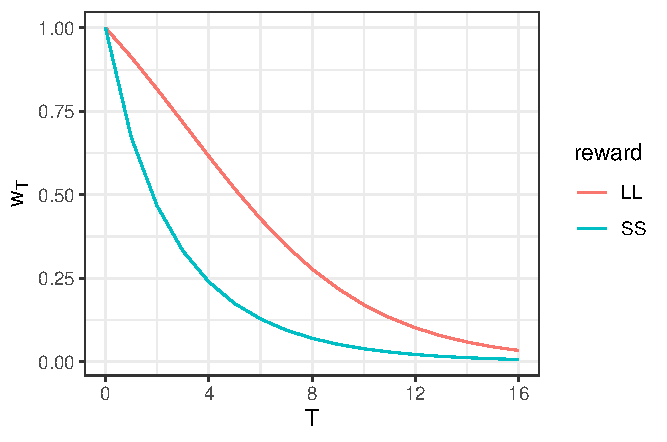
\includegraphics{images/weight_LLvSS.pdf}

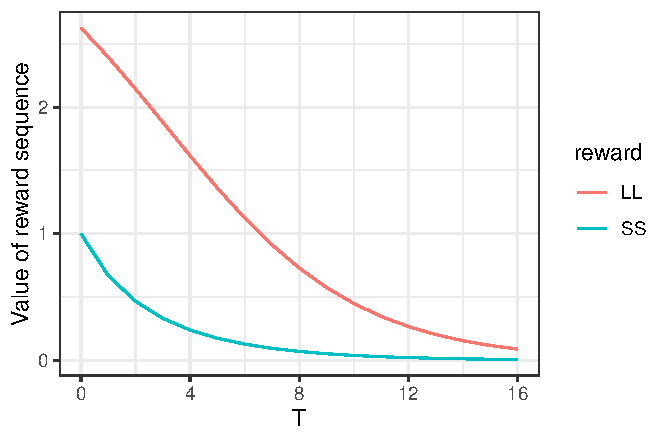
\includegraphics{images/value_LLvSS.pdf}

\hypertarget{magnitude-effect}{%
\subsection{Magnitude Effect}\label{magnitude-effect}}

The \emph{magnitude effect} is another well-known anormaly about time
preferences. Assuming we have \(t_l\), \(t_s\), \(x_s\) fixed, and want
to find a \(x_l\) such that \(V(x_l,t_l) \equiv V(x_s,t_s)\), the
magnitude effect implies that, if we increase \(x_s\), then the
\(x_l/x_s\) that makes the equality valid will decrease.

In standard discounted utility model, the magnitude effect requires the
elasticity of utility function to increase with the reward level
\citep{loewenstein_anomalies_1992}. This requirement might be too
restrictive, so that many commonly used utility functions (such as power
or CARA utility function) does not satisfy it. By contrast, in ADU
model, DM is generally assumed to attend more to periods with larger
rewards. This implies that when comparing SS and LL, she exhibits more
patience towards larger reward level, which is naturally compatible with
the magnitude effect \citep{noor_intertemporal_2011, noor_optimal_2022}.
By Proposition 3, I focus on ADU with Shannon cost function, and show
how this requirement for curvature of utility function can be relaxed in
this setting.

\textbf{Proposition 3}: \emph{Define} \(v(x)\equiv u(x)/\lambda\)
\emph{as the utility function. In ADUS, the magnitude effect always
holds true when function} \(v(x)\) \emph{satisfies}\[
RRA_v(x)\leq 1-\frac{e_v(x)}{v(x)+1}
\]\emph{where} \(RRA_v(x)\) \emph{is the relative risk aversion
coefficient of} \(v(x)\)\emph{,} \(e_v(x)\) \emph{is the elasticity of}
\(v(x)\) \emph{to} \(x\)\emph{.}

Note that Proposition 3 is a very broad condition. In Corollary 1 and
Corollary 2, I show that power utility function and CARA utility
function both satisfy this condition in most cases.

\textbf{Corollary 1}: Suppose \(v(x)=x^\gamma/\lambda\), where
\(0<\gamma<1\) and \(\lambda>0\). Then magnitude effect holds true for
any \(x\in \mathbb{R}_{>0}\).

\textbf{Corollary 2}: Suppose \(v(x)=(1-e^{-\gamma x})/\lambda\), where
\(\gamma>0\) and \(\lambda>0\). The magnitude effect holds true for any
\(x\geq \frac{1+\eta}{\gamma}\), where \(\eta>0\) and
\(\eta e^{1+\eta}-\eta=1\) (it can be calculated that
\(\eta \approx 0.35\)).

\hypertarget{concavity-of-time-discounting}{%
\subsection{Concavity of Time
Discounting}\label{concavity-of-time-discounting}}

Many time discounting models assumes discount function is convex in time
delay, e.g.~exponential and hyperbolic discounting. This style of
discount function predicts DM is \emph{risk seeking over time
lotteries}. That is, suppose a deterministic reward of level \(x\) is
delivered in period \(t_l\) with probability \(\pi\) and delivered in
period \(t_s\) with probability \(1-\pi\) (\(0<\pi<1\), \(c>0\)); while
another deterministic reward, of the same level, is delivered in a
certain period \(t_m\), where \(t_m=\pi t_l +(1-\pi) t_s\). The DM
should prefer the former reward to the latter reward. However, some
experimental studies, such as \citet{onay_intertemporal_2007} and
\citet{dejarnette_time_2020}, suggest that people are often \emph{risk
averse over time lotteries}, i.e.~preferring the reward delivered in a
certain period.

One way to accommodate the evidence about risk aversion over time
lotteries, as is suggested by \citet{dejarnette_time_2020}, is to modify
the convexity (concavity) of discount function. Under a general EDU
framework, DM is risk averse over time lotteries when
\(\pi w_{t_l}(x)+(1-\pi)w_{t_s}(x)<w_{t_m}(x)\). Fixing \(t_s\) and
\(t_l\), the inequality suggests \(w_{t_m}(c)\) is concave in \(t_m\).
In reverse, being risk seeking over time lotteries suggests
\(w_{t_m}(x)\) is convex in \(t_m\). Notably,
\citet{onay_intertemporal_2007} find that people are more likely to be
risk averse over time lotteries when \(\pi\) is small, and to be risk
seeking over time lotteries when \(\pi\) is large. Given that when
\(\pi\) gets larger, \(t_m\) is also larger, we can conclude that the
discount function may be concave in delay for the near future but convex
for the far future. Moreover, \citet{takeuchi_non-parametric_2011} also
find evidence that support this shape of discount function.

In Proposition 4, I show that ADUS can produce such a shape of discount
function as long as the reward level \(x\) is large enough.

\textbf{Proposition 4}: In ADUS, \emph{if} \(\delta =1\)\emph{, then the
discount function is convex in} \(t\)\emph{. If} \(0<\delta<1\)\emph{,
then there are a reward threshold} \(\underline{x}\) \emph{and a time
threshold} \(\underline{t}\) \emph{such that}

\begin{enumerate}
\def\labelenumi{\arabic{enumi})}
\tightlist
\item
  \emph{when} \(x\leq \underline{x}\)\emph{, the discount function is
  convex in} \(t\)\emph{;}
\item
  \emph{when} \(x > \underline{x}\)\emph{, the discount function is
  convex in} \(t\) \emph{given} \(t\geq \underline{t}\)\emph{, and it is
  concave in} \(t\) \emph{given} \(t<\underline{t}\)\emph{.}
\end{enumerate}

\emph{It can be derived that}
\(v(\underline{x})=\ln(\frac{2}{1-\delta})\)\emph{, and}
\(\underline{t}=\frac{\ln[(1-\delta)e^{v(x)}-1]}{-\ln\delta}\)\emph{.}

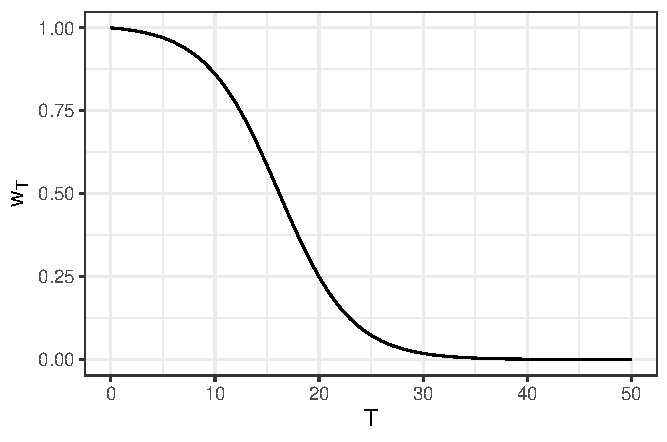
\includegraphics{images/concavity_discount.pdf}

\hypertarget{s-shaped-value-function}{%
\subsection{S-Shaped Value Function}\label{s-shaped-value-function}}

In prospect theory, \citet{kahneman_prospect_1979} propose an S-shaped
value function that is convex for losses and concave for gains. Since
that, S-shaped value functions have been widely embraced by behavioral
economists. More recent theories have provided further justifications
for it, including reference-dependent utility in a broad sense
\citep{koszegi_model_2006}, and efficient coding of values
\citep{frydman_efficient_2021}. Here, I provide an account based on
selective attention to time periods.

Suppose a DM is faced with a choice between a risky lottery and a fixed
amount of money. When making this choice, she does not obtain any money
from either option. Thus, she perceives the outcome of each option as
something that will happen in the future. She allocate her attention
between the present period and the period when she may receive the
money. Assume that she perceives the outcome will be realized in period
\(t\), and in a certain state, the option she chooses yields reward
\(x\), then we can use the attentional discounted utility \(V(x,t)\) to
represent the value function. I derive the conditions in which ADUS can
produce a S-shaped value function in Proposition 5.

\textbf{Proposition 5}: \emph{Suppose} \(t\geq1\)\emph{,}
\(\frac{d}{dx}\left(\frac{1}{v'(x)}\right)\) \emph{is continuous in}
\((0,+\infty)\)\emph{, in ADUS,}

\begin{enumerate}
\def\labelenumi{\arabic{enumi})}
\item
  \emph{there exists a threshold} \(\bar{x}\) \emph{in} \((0,+\infty)\)
  \emph{such that} \(V(x,t)\) \emph{is strictly concave in} \(x\)
  \emph{when} \(x\in [\bar{x},+\infty)\)\emph{;}
\item
  \emph{if} \(\frac{d}{dx}\left(\frac{1}{v'(x)}\right)\) \emph{is
  right-continuous at} \(x=0\)\emph{, and}
  \(\frac{d}{dx}\left(\frac{1}{v'(0)}\right)<1\)\emph{, then there
  exists a threshold} \(x^*\) \emph{in} \((0, \bar{x})\) \emph{such
  that, for any} \(x\in (0,x^*)\)\emph{,} \(V(x,t)\) \emph{is strictly
  convex in} \(x\)\emph{;}
\item
  \emph{there exist a hyper-parameter} \(\lambda^*\) \emph{and an
  interval} \((x_1,x_2)\) \emph{such that, if}
  \(\lambda<\lambda^*\)\emph{, for any} \(x\in(x_1,x_2)\)\emph{,}
  \(V(x,t)\) \emph{is strictly convex in} \(x\)\emph{, where}
  \(\lambda^*>0\) \emph{and} \((x_1,x_2)\subset(0,\bar{x})\)\emph{.}
\end{enumerate}

Proposition 5 implies, if the derivative of \(\frac{1}{v'(x)}\)
converges to a small number when \(x\rightarrow 0^+\), or the unit cost
of information \(\lambda\) is small enough, value function \(V(x,t)\)
will perform an S shape in some interval of \(x\). At the intuition
level, note that \(V(x,t)=w_t(x)v(x)\). When the level of reward \(x\)
grows, both the instantaneous utility of it, i.e.~\(v(x)\), and the
discounting factor assigned to it, i.e.~\(w_t(x)\), can increase. These
functions are both concave in \(x\): when the level of reward is small,
they both grow fast. So, it is possible that their product is convex in
this case. By contrast, when the level of reward is large, they grow
slowly, so their product keeps concave.

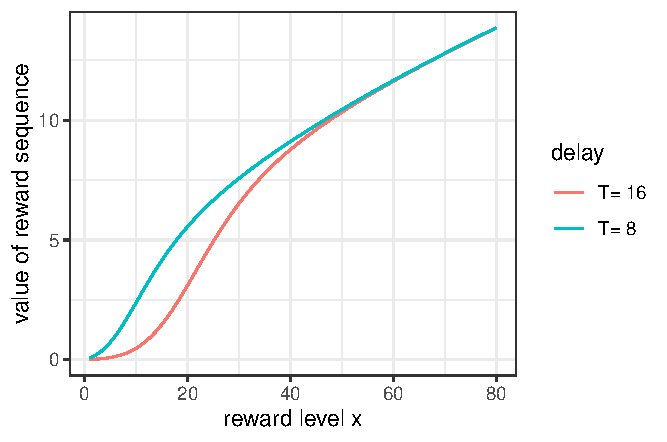
\includegraphics{images/S_shaped_value.pdf}

\hypertarget{inseparability-of-sequences}{%
\subsection{Inseparability of
Sequences}\label{inseparability-of-sequences}}

Let \(x\) and \(y\) denote two 2-period risky reward sequences. For
\(x\), the realized sequence is {[}£100,£100{]} with probability 1/2,
and is {[}£3,£3{]} with probability 1/2. For \(y\), the realized
sequence is {[}£3,£100{]} with probability 1/2, and is {[}£100,£3{]}
with probability 1/2. Classical models of intertemporal choice typically
assume the separability of potentially realized sequences. This implies
that the DM is indifferent between \(x\) and \(y\). However,
\citet{andersen_multiattribute_2018} find evidence of
\emph{intertemporal correlation aversion}, that is, people often prefer
\(y\) to \(x\).

ADU can naturally yield intertemporal correlation aversion. For
simplicity, suppose the initial attention is uniformly distributed
across the two periods. For \(x\), under each potentially realized
sequence, the DM equally weights each period. For \(y\), DM tends to
assign more weight to the period with a reward of £100 (suppose that
weight is \(w\)). Then the value of \(x\) is
\(\frac{1}{2} u(100) + \frac{1}{2} u(3)\) and the value of \(y\) is
\(w\cdot u(100) +(1-w) \cdot u(3)\). Given that \(x>\frac{1}{2}\), the
DMs should strictly prefer \(y\) to \(x\).

\begin{itemize}
\tightlist
\item
  Other evidence related to inseparability: common sequence effect,
  (reverse) mere token effect, magnitude-increasing temporal sensitivity
\end{itemize}

\hypertarget{the-role-of-attention-in-inconsistent-planning}{%
\section{The Role of Attention in Inconsistent
Planning}\label{the-role-of-attention-in-inconsistent-planning}}

\hypertarget{attention-grabbing-and-updating}{%
\subsection{Attention Grabbing and
Updating}\label{attention-grabbing-and-updating}}

Suppose a DM has budget \(m\) (\(m>0\)) and is considering how to spend
it over different time periods. We can use a reward sequence \(x\) to
represent this decision problem, where the DM's spending in period \(t\)
is \(x_t\). In period 0, she wants to find a \(x\) such
that\[ \tag{3} \max_{x}\;\sum_{t=0}^T w_t u(x_t)\quad s.t. \;\sum_{t=0}^T x_t = m   \]

where \(w_t\) is the attention-adjusted discounting factor in period
\(t\). I assume
\(w_t=\delta^t e^{u(x_t)/\lambda}/\sum_{t=\tau}^T \delta^{\tau} e^{u(x_\tau)/\lambda}\)
and there is no risk under this setting.

In models like exponential and hyperbolic discounting, the discounting
factor of a future period is consistently smaller than that of the
current period. Thus, the DM should spend more at the present than in
the future. By contrast, in ADU, when increasing the spending in a
certain period, the discounting factor corresponding to that period
should also increase. So it is possible that the DM spends more in the
future and that a future period has a greater discounting factor than
the current period. This is consistent with
\citet{loewenstein_preferences_1993} that find people sometimes prefer
improving sequences to declining sequences.

ADU suggests there are two mechanisms that can help explain why people
may perform dynamically inconsistent behavior. The first is
\emph{attention-grabbing effect}, that is, keeping the others equal,
when we increase \(x_t\) (which lead to an increase in \(w_t\)), the
discounting factor in any other period should decrease due to limited
attention. After omitting a previous period from the decision problem in
Equation (3), the DM can assign more weights to remaining periods; thus,
the attention-grabbing effect is enhanced. The increased
attention-grabbing effect will offset some benefit of increasing
spending toward a certain period. Therefore, when the DM prefers
improving sequences, the attention-grabbing effect will make her perform
a present bias-like behavior (always feeling that she should spend more
at the present than the original plan); when the DM prefers declining
sequences, this effect will maker her perform a future bias-like
behavior (always feeling she should spend more in the future).

The second mechanism is \emph{initial attention updating}. As is assumed
above, in period 0, prior to evaluating each reward sequence, the DM's
initial weight on period \(t\) is proportional to \(\delta^t\); after
evaluation, the weight becomes being proportional to
\(\delta^t e^{u(x_t)/\lambda}\). In period 1, if she implements the
evaluation based on the information attained in period 0, the initial
weight should be updated to being proportional
\(\delta^t e^{u(x_t)/\lambda}\); thus, the weight after evaluation
should become being proportional to \(\delta e^{2u(x_t)/\lambda}\). As a
result, the benefit of increasing spending toward a certain period gets
strengthened. The updated initial attention can make those who prefer
improving sequences perform present bias and those who prefer declining
sequences perform future bias.

Both the attention-grabbing effect and initial attention updating are
affected by the curvature of utility function. They jointly decide which
behavior pattern that people should perform in dynamics.

\textbf{Proposition 6} (\emph{spread-consistency correlation}) Suppose
\(\succsim\) has a ADU representation and satisfies Axiom 2-4. If there
exist \(b\) and \(S_T\) such that, for any \(b'\) and \(S_T'\),
\(bS_T\succsim b'S_T'\), where
\(b+\sum_{t=0}^Ts_t=b'+\sum_{t=0}^Ts_t'\), then for any \(S'_T\), we
have \[S_T \succsim S_T' \Longleftrightarrow b\sim S_T\]where
\(\sum_{t=0}^Ts_t=\sum_{t=0}^Ts_t'\).

Proposition 6 implies that, when allocating a consumption budget across
time periods, the DM keeps her choice dynamically consistent if and only
if she performs a strong preference for spread. Given that people are
typically assumed to be impatient (preferring a declining sequence), one
intuitive interpretation of Lemma 2 is that the less impatient a DM is
in the present, the less inclined she is to deviate from the original
choice in the future.

\hypertarget{discussion}{%
\section{Discussion}\label{discussion}}

\hypertarget{relation-to-other-models-of-intertemporal-choices}{%
\subsection{Relation to Other Models of Intertemporal
Choices}\label{relation-to-other-models-of-intertemporal-choices}}

The theory most similar to AAD is the salience theory
\citep{bordalo2012salience, bordalo2013salience, bordalo2020memory}.

rational inattention

focus-weighted utility

bayesian updating and discounting

optimal precision

Relation with money/delay trade-off

\hypertarget{other-relevant-phenomena}{%
\subsection{Other relevant phenomena}\label{other-relevant-phenomena}}

\hypertarget{limitation}{%
\subsection{Limitation}\label{limitation}}

attention biases learning: learning rate is high for attended reward

\hypertarget{conclusion}{%
\section{Conclusion}\label{conclusion}}

\renewcommand\refname{Reference}
  \bibliography{reference.bib}

\newpage

\hypertarget{appendix}{%
\section{Appendix}\label{appendix}}

\hypertarget{a.-proof-of-proposition-1}{%
\subsection{A. Proof of Proposition 1}\label{a.-proof-of-proposition-1}}

The sufficiency is easy to validate. We present the proof of necessity
here. That is, if \(\succsim\) has an optimal discounting representation
and satisfies Axiom 1-4, then it has an AAD representation.

\noindent \textbf{Lemma 1}: \emph{If Axiom 1 and 3 hold, for any}
\(s_{0\rightarrow T}\)\emph{, there exist} \(w_0, w_1, …, w_T > 0\)
\emph{such that}
\(s_{0\rightarrow T} \sim w_0 \cdot s_0 + ...+w_T\cdot s_T\)\emph{,
where} \(\sum_{t=0}^T w_t=1\)\emph{.}

\noindent \emph{Proof}: If \(T=1\), Lemma 1 is a direct application of
Axiom 3. If \(T\geq 2\), for any \(2\leq t\leq T\), there should exist
\(\alpha_t\in(0,1)\) such that
\(s_{0\rightarrow t}\sim \alpha_t\cdot s_{0\rightarrow t-1}+(1-\alpha_t)\cdot s_{t}\).
By state-independence and reduction of compound alternatives, we can
recursively apply this equivalence relation as follows:\[
\begin{aligned}
s_{0\rightarrow T} &\sim \alpha_{T-1}\cdot s_{0\rightarrow T-1} + (1-\alpha_{T-1})\cdot s_T \\
&\sim  \alpha_{T-1}\alpha_{T-2}\cdot s_{0\rightarrow T-2} + \alpha_{T-1}(1-\alpha_{T-2})\cdot s_{T-1} + (1-\alpha_{T-1})\cdot s_T \\
& \sim ...\\
& \sim w_0 \cdot s_0 + w_1\cdot s_1 +... +w_T\cdot s_T
\end{aligned}
\]where \(w_0=\prod_{t=0}^{T-1}\alpha_t\), \(w_T = 1-\alpha_{T-1}\), and
for \(0<t<T\),
\(w_t=(1-\alpha_{t-1})\prod_{\tau=t}^{T-1}\alpha_{\tau}\). It is easy to
show the sum of \(w_0,…,w_T\) is equal to 1. \emph{QED}.

Therefore, if Axiom 1 and 3 hold, for any reward sequence
\(s_{0\rightarrow T}\), we can always find a convex combination of all
its elements, such that the DM is indifferent between the reward
sequence and this convex combination. If \(s_{0\rightarrow T}\) is a
constant sequence, i.e.~all its elements are constant, then we can
directly assume \(\mathcal{W}\) is AAD-style. Henceforth, we discuss
whether AAD can also apply to non-constant sequences.

By Lemma 2, we show adding a new reward to the end of
\(s_{0\rightarrow T}\) has no impact on the relative decision weights of
rewards in the original reward sequence.

\noindent \textbf{Lemma 2}: \emph{For any}
\(s_{0\rightarrow T+1}\)\emph{, if}
\(s_{0\rightarrow T}\sim \sum_{t=0}^T w_t \cdot s_t\) \emph{and}
\(s_{0\rightarrow T+1} \sim \sum_{t=0}^{T+1} w'_t\cdot s_t\)\emph{,
where} \(w_t, w'_t>0\) and \(\sum_{t=0}^Tw_t=1\)\emph{,}
\(\sum_{t=0}^{T+1}w'_t=1\)\emph{, then when Axiom 1-4 hold, we can
obtain} \(\frac{w'_0}{w_0}=\frac{w'_1}{w_1}=…=\frac{w'_T}{w_T}\)\emph{.}

\noindent \emph{Proof}: According to Axiom 3, for any
\(s_{0\rightarrow T+1}\), there exist \(\alpha,\zeta \in (0,1)\) such
that\[\tag{A1}
\begin{aligned}
s_{0 \rightarrow T}\sim\alpha\cdot s_{0 \rightarrow T-1} + (1-\alpha)\cdot s_T \\
s_{0\rightarrow T+1} \sim \zeta\cdot s_{0\rightarrow T} + (1-\zeta)\cdot s_{T+1}
\end{aligned}
\]On the other hand, we drawn on Lemma 1 and set\[\tag{A2}
s_{0\rightarrow T+1} \sim \beta_0\cdot s_{0 \rightarrow T-1} + \beta_1\cdot s_T + (1-\beta_0-\beta_1)\cdot s_{T+1}
\]where \(\beta_0, \beta_1 > 0\). According to Axiom 4,
\(1-\zeta=1-\beta_0-\beta_1\). So, \(\beta_1=\zeta-\beta_0\). This also
implies \(\zeta > \beta_0\).

According to Axiom 2, we suppose there exists a reward sequence \(s\)
such that
\(s \sim \frac{\beta_0}{\zeta}\cdot s_{0 \rightarrow T-1} + (1-\frac{\beta_0}{\zeta})\cdot s_1\).
By Equation (A2) and reduction of compound alternatives, we have
\(s_{0\rightarrow T+1}\sim \zeta \cdot s + (1-\zeta)\cdot s_{T+1}\).
Combining Equation (A2) with the second line of Equation (A1) and
applying transitivity and state-independence, we obtain
\(s_{0\rightarrow T} \sim \frac{\beta_0}{\zeta}\cdot s_{0 \rightarrow T-1} + (1-\frac{\beta_0}{\zeta})\cdot s_1\).

We aim to prove that for any \(s_{0\rightarrow T+1}\), we can obtain
\(\alpha=\frac{\beta_0}{\zeta}\). To do this, we first assume (without
loss of generality) that \(\alpha > \frac{\beta_0}{\zeta}\).

Consider the case that \(s_{0 \rightarrow T-1} \succ s_T\). By
state-independence, for any \(c\in \mathbb{R}_{\geq 0}\), we have
\((\alpha - \frac{\beta_0}{\zeta})\cdot s_{0\rightarrow T-1} + (1-\alpha+\frac{\beta_0}{\zeta})\cdot c \succ (\alpha - \frac{\beta_0}{\zeta})\cdot s_T + (1-\alpha+\frac{\beta_0}{\zeta})\cdot c\).
By Axiom 2, there exists \(z\in \mathbb{R}_{\geq 0}\) such that
\((1-\alpha)\cdot s_T + \frac{\beta_0}{\zeta}\cdot s_{0\rightarrow T-1}\sim z\).
Given \(c\) is arbitrary, we set
\((1-\alpha+\frac{\beta_0}{\zeta})\cdot c \sim z\). By reduction of
compound alternatives, we can derive that\[
(\alpha-\frac{\beta_0}{\zeta})\cdot s_{0\rightarrow T-1} +(1-\alpha)\cdot s_T + \frac{\beta_0}{\zeta}\cdot s_{0\rightarrow T-1} \succ (\alpha-\frac{\beta_0}{\zeta})\cdot s_T +(1-\alpha)\cdot s_T + \frac{\beta_0}{\zeta}\cdot s_{0\rightarrow T-1}
\]where the LHS can be rearranged to
\(\alpha\cdot s_{0\rightarrow T-1} + (1-\alpha)\cdot s_T\), and the RHS
can be rearranged to
\(\frac{\beta_0}{\zeta}\cdot s_{0 \rightarrow T-1} + (1-\frac{\beta_0}{\zeta})\cdot s_1\).
They both should be indifferent from \(s_{0\rightarrow T}\). This
results in a contradiction. Similarly, in the case that
\(s_T \succ s_{0 \rightarrow T-1}\), we can also derive a contradiction.
Meanwhile, when \(s_{0\rightarrow T}\sim s_T\), \(\alpha\) and
\(\frac{\beta_0}{\zeta}\) can be any number within \((0,1)\). So, we can
directly set \(\alpha = \frac{\beta_0}{\zeta}\).

Thus, we have \(\alpha = \frac{\beta_0}{\zeta}\) for any
\(s_{0\rightarrow T+1}\), which indicates
\(\frac{\beta_0}{\alpha}=\frac{\beta_1}{1-\alpha}=\zeta\). We can
recursively apply this equality to any sub-sequence
\(s_{0\rightarrow t}\) (\(t\leq T\)) of \(s_{0\rightarrow T+1}\), so
that the lemma will be proved. \emph{QED}.

Now we move on to prove Proposition 1. The proof contains five steps.

First, we add the constraints \(\sum_{t=0}^T w_t=1\) and \(w_t>0\) to
the optimal discounting problem for \(s_{0\rightarrow T}\) so that the
problem is compatible with Lemma 1. According to the FOC of its
solution, for all \(t=0,1,….,T\), we have\[\tag{A3}
f_t'(w_t)=u(s_t)+\theta
\]where \(\theta\) is the Lagrange multiplier. Given that \(f'_t(w_t)\)
is strictly increasing, \(w_t\) is increasing with \(u(s_t)+\theta\). We
define the solution as \(w_t =\phi_t(u(s_t)+\theta)\).

Second, we add a new reward \(s_{T+1}\) to the end of
\(s_{0\rightarrow T}\) and apply Lemma 2 as a constraint to optimal
discounting problem. Look at the optimal discounting problem for
\(s_{0\rightarrow T+1}\). For all \(t\leq T\), the FOC of its solution
will take the same form as Equation (A3). So, if importing \(s_{T+1}\)
changes some \(w_t\) to \(w'_t\) (\(w'_t \neq w_t\), where \(w_t\) is
the solution to optimal discounting problem for \(s_{0\rightarrow T}\)),
the only way is through changing the multiplier \(\theta\). Suppose
importing \(s_{T+1}\) changes \(\theta\) to \(\theta-\Delta \theta\), we
have \(w'_t = \phi_t(u(s_t)+\theta-\Delta \theta)\).

By Lemma 2, we know
\(\frac{w_0}{w'_0}=\frac{w_1}{w'_1}=…=\frac{w_T}{w'_T}\). In other
words, for \(t=0,1,…,T\), we have
\(w_t \propto \phi_t(u(s_t)+\theta-\Delta \theta)\). We can rewrite
\(w_t\) as \[\tag{A4}
w_t = \frac{\phi_t(u(s_t)+\theta-\Delta \theta)}{\sum_{\tau=0}^{T}\phi_\tau(u(s_\tau)+\theta-\Delta \theta)}
\]

Third, we show that in \(s_{0\rightarrow T}\), if we change each \(s_t\)
to \(z_t\) such that \(u(z_t)=u(s_t)+\Delta u\), the decision weights
\(w_0,…,w_T\) will remain the same. Note
\(\sum_{t=0}^T \phi_t(u(s_t)+\theta)=1\). It is clear that
\(\sum_{t=0}^T \phi_t(u(z_t)+\theta-\Delta u)=1\). Suppose changing
every \(s_t\) to \(z_t\) moves \(\theta\) to \(\theta'\) and
\(\theta'<\theta-\Delta u\). Then, we must have
\(\phi_t(u(z_t)+\theta')<\phi_t(u(z_t)+\theta-\Delta u)\) since
\(\phi_t(.)\) is strictly increasing. This results in
\(\sum_{t=0}^T \phi_t(u(z_t)+\theta')<1\), which contradicts with the
constraint that the sum of all decision weights is 1. The same
contradiction can apply to the case that \(\theta'>\theta-\Delta u\).
Therefore, changing every \(s_t\) to \(z_t\) must move \(\theta\) to
\(\theta - \Delta u\), and each \(w_t\) can only be moved to
\(\phi_t(u(z_t)+\theta -\Delta u)\), which is exactly the same as the
original decision weight.

A natural corollary of this step is that, subtracting or adding a common
number to all intantaneous utilities in a reward sequence has no effect
on decision weights. What actually matters for determining the decision
weights is the difference between instantaneous utilities. This
indicates, for convenience, we can subtract or add an arbitrary number
to the utility function.

In other words, for a given \(s_{0\rightarrow T}\) and \(s_{T+1}\), we
can define a new utility function \(v(.)\) such that
\(v(s_t) = u(s_t) +\theta-\Delta \theta\). So, Equation (A4) can be
re-written as\[
w_t = \frac{\phi_t(v(s_t))}{\sum_{\tau=0}^{T}\phi_\tau(v(s_\tau))}
\]If \(w_t\) takes the AAD form under the utility function \(v(.)\),
i.e.~\(w_t \propto d_t e^{v(s_t)/\lambda}\), then it should also take
the AAD form under the original utility function \(u(.)\).

Fourth, we show \(\Delta \theta\) has two properties: (i)
\(\Delta \theta\) is strictly increasing with \(u(s_{T+1})\); (ii)
suppose \(\Delta \theta = \underline{\theta}\) when
\(u(s_{T+1})=\underline{u}\) and \(\Delta\theta=\bar{\theta}\) when
\(u(s_{T+1})=\bar{u}\), where \(\underline{u}<\bar{u}\), then for any
\(l \in(\underline{\theta},\bar{\theta})\), there exists
\(u(s_{T+1})\in(\underline{u},\bar{u})\) such that
\(\Delta \theta = l\).

The property (i) can be shown by contradiction. Given \(w_0,…,w_{T+1}\)
a sequence of decision weights for \(s_{0\rightarrow T+1}\). Suppose
\(u(s_{T+1})\) is increased but \(\Delta \theta\) is constant. In this
case, each of \(w'_0,…,w'_T\) should also be constant. However,
\(w'_{T+1}\) must increase as it is stricly increasing with
\(u(s_{T+1})+\theta-\Delta \theta\) (\(\theta\) is determined by the
optimal discounting problem for \(s_{0\rightarrow T}\); thus, any
operations on \(s_{T+1}\) should have no effect on \(\theta\)). This
contradicts with the constraint that \(\sum_{t=0}^{T+1} w'_t =1\). The
only way to avoid such contradictions is to set \(\Delta \theta\)
strictly increasing with \(s_{T+1}\), so that \(w'_0,…,w'_T\) are
decreasing with \(u(s_{T+1})\).

For property (ii), note that for any reward sequence
\(s_{0\rightarrow T+1}\) and a given \(\theta\), \(\Delta\theta\) is
defined as the solution to
\(\sum_{t=0}^{T+1} \phi_t(u(s_t)+\theta-\Delta\theta)=1\). Given an
arbitrary number \(l\in(\underline{\theta},\bar{\theta})\), the proof of
property (ii) consists of two stages. First, for \(t=0,1,…,T\), we need
to show that \(u(s_t)+\theta-l\) is still in the domain of
\(\phi_t(.)\). Second, for period \(T+1\), we need to show for any
\(\omega\in(0,1)\), there exists \(u(s_{T+1})\in \mathbb{R}\) such that
\(\phi_{T+1}(u(s_{T+1})+\theta-l)=\omega\).

For the first stage, note \(\phi_t(.)\) is the inverse function of
\(f'_t(.)\). Suppose when \(\Delta\theta=\underline{\theta}\), we have
\(f'_t(w^{a}_t)=u(s_t)+\theta-\underline{\theta}\), and when
\(\Delta\theta=\bar{\theta}\), we have
\(f'_t(w^{b}_t)=u(s_t)+\theta-\bar{\theta}\). For any
\(l\in(\underline{\theta},\bar{\theta})\), we have
\(u(s_t)+\theta-l \in (f'_t(w^b_t),f'_t(w^a_t))\). Given that
\(f'_t(.)\) is continuous and strictly increasing, there must be
\(w_t\in(w^b_t,w^a_t)\) such that \(f'_t(w_t)=u(s_t)+\theta-l\). So,
\(u(s_t)+\theta-l\) is in the domain of \(\theta_t(.)\). For the second
stage, given an arbitrary \(\omega\in(0,1)\), we can set
\(u(s_{T+1})=f'(\omega)-\theta+l\), so that the desired condition is
satisfied.

A corollary of this step is that we can manipulate \(\Delta \theta\) in
Equation (A4) at any level in \([\underline{\theta},\bar{\theta}]\) by
changing a hypothetical \(s_{T+1}\).

Fifth, we show \(\ln \phi_t(.)\) is linear under some conditions. To do
this, let us add a hypothetical \(s_{T+1}\) to the end of \(s_T\) and
let \(w'_t=\phi_t(v(s_t))\) denote the decision weights for
\(t=0,1,…,T+1\) in \(s_{0\rightarrow T+1}\). We change the hypothetical
\(s_{T+1}\) within the set
\(\{s_{T+1}|u(s_{T+1})\in[\underline{u},\bar{u}]\}\) and see what will
happen to the decision weights from period 0 to period \(T\). Suppose
this changes each \(w'_t\) to \(\phi_t(v(s_t)+\theta')\). Set
\(\theta'=a\) when \(u(s_{T+1})=\underline{u}\) and \(\theta'=b\) when
\(u(s_{T+1})=\bar{u}\). By the second step, we have\[\tag{A5}
\frac{\phi_t(v(s_t))}{\sum_{\tau=0}^{T}\phi_\tau(v(s_\tau))} = \frac{\phi_t(v(s_t)+\theta')}{\sum_{\tau=0}^{T}\phi_\tau(v(s_\tau)+\theta')}
\]For each \(t=0,1,...,T\), we can rewrite \(\phi_t(v(s_t))\) as
\(e^{\ln \phi_t(v(s_t))}\). For the LHS of Equation (A5), multiplying
both the numerator and the denominator by a same number will not affect
the value. Therefore, Equation (A5) can be rewritten as \[
\frac{e^{\ln\phi_t(v(s_t))+\kappa\theta'}}{\sum_{\tau=0}^{T}e^{\ln\phi_\tau(v(s_\tau))+\kappa\theta'}} = \frac{e^{\ln\phi_t(v(s_t)+\theta')}}{\sum_{\tau=0}^{T}e^{\ln\phi_\tau(v(s_\tau)+\theta')}}
\]where \(\kappa\) can be any real-valued constant. By properly
selecting \(\kappa\), we can obtain
\(\ln \phi_t(v(s_t))+\kappa\theta'=\ln \phi_t(v(s_t)+\theta')\) for all
\(t=0,1,...,T\). And if \(\theta'>0\), we must have \(\kappa>0\).

This indicates a property of function \(\ln \phi_t(.)\): for any
\(v\in \mathbb{R}\), we have
\(\ln \phi_t(v)=\ln \phi_t(v-\theta')+\kappa\theta'\) as long as
\(\theta' \in [a,b]\).

So, we can write \(\ln \phi_t (u(s_t))\) as
\(\ln \phi_t(u(0))+\lambda u(s_t)\)

\end{document}
